\resetfigpath{ksp}
\glsresetall

\section{Multi-path tracking}
This section gives a theoretical background to the multi-path tracking problem, as first developed in \cite{berclaz11}.
The latter framework is leveraged in our first major contribution, where we perform tracking of over-segmented regions across a sequence, where each region can be part of object of interest.

We develop our multi-path tracking framework through the following steps.
(1) We first represent our sequence as a stack of occupancy grid, where each element of a grid represent an over-segmented region.
The elements of these grids are then represented as the nodes of a directed acyclic graph, connected by edges that represent admissible motions.
(2) We introduce the notion of discrete flow variables, which represent the number of objects passing from one position of the grid to another.
(3) We formulate the multi-path tracking problem as a \gls{map} problem, where the grid occupancies are binary random variables.
(4) We show how the latter problem, under the Markov assumption, is identical to an \gls{ip}.
(5) As the latter is NP hard, we show that relaxing it to a continuous \gls{lp} and solving it using off-the-shelf solvers converges to the optimal solution.
(6) We further show that the implicit spatio-temporal relations of our occupancy grid allow to leverage the \gls{ksp} algorithm.

Formally, we start by formulating our problem in the network-flow paradigm.
Next, we show the latter allow to solve a \gls{map} problem, where the objectness of over-segmented regions are the variables to optimize, and show how the likelihoods can be modeled by appearance similarity models.
Last, we show how solving the latter \gls{map}, when cast into a network flow problem, can be solved efficiently.

\subsection{Segmentation as a network flow problem on over-segmented regions}
We depart from the work of \cite{berclaz11} on two aspects: (1) In contrast to the latter authors, who represent a sequence as a stack of coarse grids, i.e. each cell represent a physical position and the relative locations are fixed in advance, we rather consider that our sequence is over-segmented into superpixels.
(2) We leverage the ``tracklet'' paradigm, where each over-segmented region is represented as a short track in which flow is allowed to pass through.


In particular, we generate on each frame, indexed by a time variable $t$, a set of $N_{t}$ non-overlapping over-segmented regions $\mathcal{S}_{t}=\{s_{t}^{n}\}_{n=1}^{N_{t}}$.
Within the directed graph representation, we represent each over-segmented region $s^{t}_{n}$ by a couple of nodes connected by a \textit{visiting} edge $e^{n}_{t}$.
As a side note, the latter is often referred to as a ``tracklet'' \cite{zhang08}.
So as to allow objects to transit from one frame to the next, we add \textit{transition} edges $e^{(n,m)}_{t}$ that connect region $s^{n}_{t}$ to region $s^{m}_{t+1}$.
Each edge is labeled with a discrete non-negative flow variable.
In particular, $f_{t}^{n}$ corresponds to the flow transiting through edge $e_{t}^{n}$, while $f_{t}^{n,m}$ corresponds to the flow passing from region $s_{t}^{n}$ to region $s_{t+1}^{m}$.
Next, we impose conservation of flow, which imposes that the quantity of flow that passes into a visiting edge is equal to the quantity of flow that leaves it. Formally:

\begin{equation}
  \label{eq:flow_conserv}
  \forall t,n \quad f_{t}^{n} = \sum_{n:m\in \mathcal{N}(n)}f_{t}^{n,m}
\end{equation}

When $\mathcal{N}(n)$ is a spatial neighborhood centered on region $n$ that defines admissible motion.

Next, as we assume that each region can contain a maximum of one object. Formally:

\begin{equation}
  \label{eq:capa_constrain}
  \forall t,n \quad f_{t}^{n} \leq 1
\end{equation}

Note that Eq. \ref{eq:flow_conserv} and \ref{eq:capa_constrain} implicitly enforce a maximum flow constraint on transition edges.

At the root of our segmentation framework lies the basic idea that our object to segment is composed of over-segmented regions that are spatially and temporally organized.
Moreover, we expect that the size of our object of interest changes through time/slice, e.g. a brain tumor on transversal slices appears to grow and shrink again as one scrolls from one end of the scan to the other end.
To address this requirement, we introduce two kinds of \textit{virtual} nodes: A source node and a sink node.
The first acts like a tap, i.e. it pushes flow inside the graph and increases the total mass, while the second allows to evacuate mass.
We ensure a flow-mass conservation through the constraint:

\begin{equation}
  \label{eq:mass_constrain}
  \sum_{t,m\in \mathcal{N}(\xi_{t})}f_{xi_{t},m} = \sum_{k:\mathcal{X}\in\mathcal{N}(k)}f^{t}_{k,\mathcal{X}}
\end{equation}

Where the $\xi_{t}$ are proxy source nodes that allow pushing flow on frame $t$, and $\mathcal{X}$ is the sink node.
Fig. \ref{fig:flownetwork} illustrates our network flow.

\begin{figure}[!htpb]
  \centering
  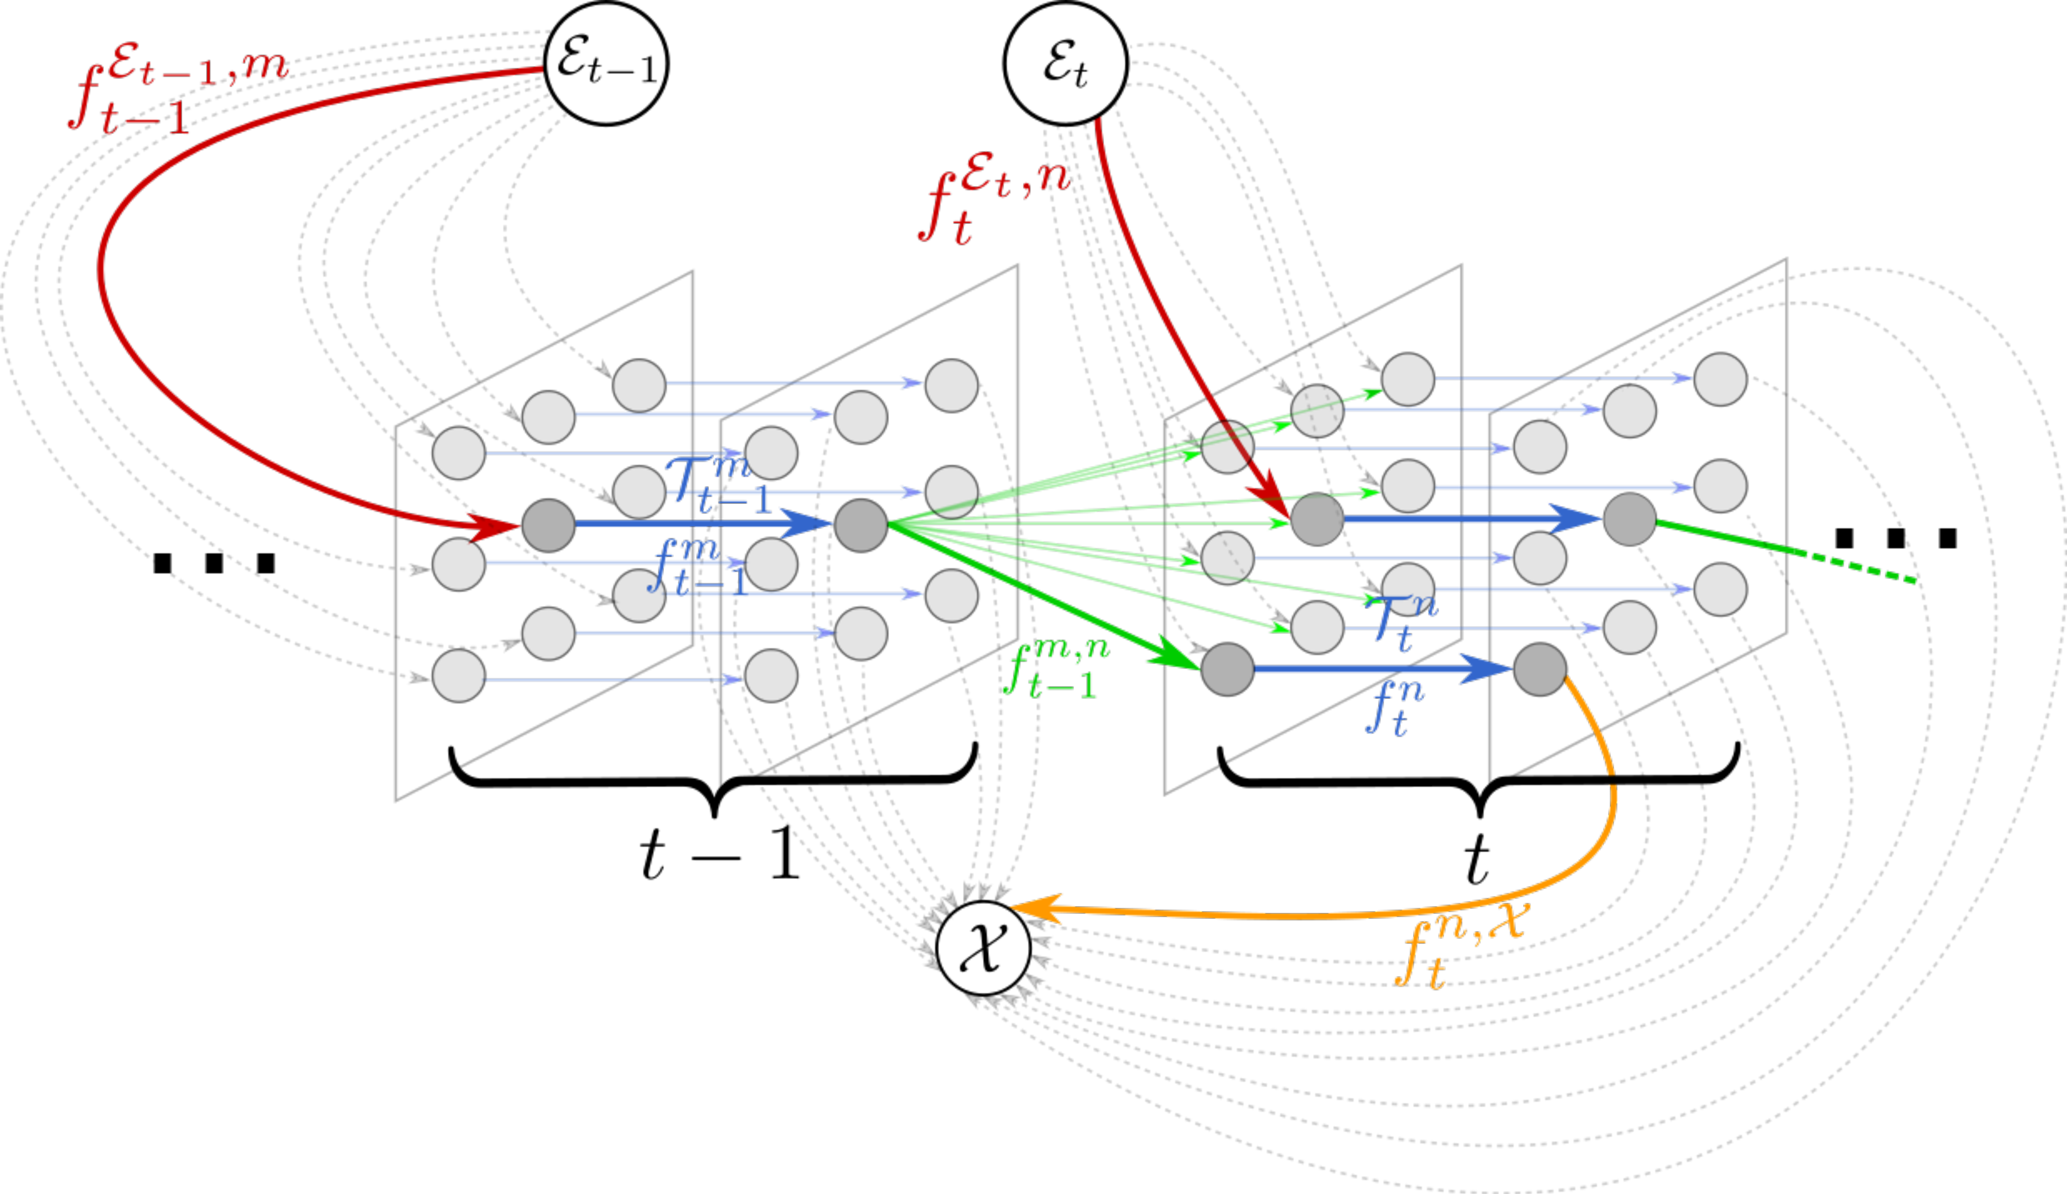
\includegraphics[width=13cm]{fig3}
  \caption{Illustration of our flow network. Each over-segmented region is assigned a visiting edge (in blue).
    Flow is allowed to pass from one frame to the next through the transition edges (in green).
    A set of proxy source nodes $\xi_{t}$ allow to push flow into the network through entrance edges (in red).
  The sink node $\mathcal{X}$ allows to evacuate flow through exit edges (in orange).}
  \label{fig:flownetwork}
\end{figure}

\subsection{Maximum a Posteriori formulation}
We first formulate an \gls{map} estimation problem, where the random variable to optimize for denotes the presence of objects at discrete time-space locations.
Next, we emphasize how the network flow paradigm developed above is leveraged in order to solve the \gls{map} estimation problem.

Let $\bm{Y}={Y^{n}_{t}|\forall(t,n)}$ a set of binary random variable that take value $1$ when region $s^{n}_{t}$ is object, and $0$ otherwise, while $\bm{I}_{t=1}^{N}$ and $\bm{g}_{t=1}^{N}$ are a set of $N$ images and user-provided 2D locations, respectively.
We define our segmentation task as.

\begin{equation}
  \label{eq:map}
  y^{*} = \arg \max_{y \in \mathcal{Y}}P(\bm{Y}=\bm{y}|\bm{I}, \bm{g})
\end{equation}

where $y^{*}$ are the optimal binary labels.
Assuming that $Y^{t}_{n}$ is conditionally independent given the observed variables, we rewrite Eq. \ref{eq:map} as

\begin{equation}
  \label{eq:bg_map2}
  y^{*} = \arg \max_{y \in \mathcal{Y}}\prod_{i,j,t} P_{visit}(Y^{t}_{n}|\bm{I}, \bm{g}) P_{trans}(Y^{t}_{n}|I^{t-1},\bm{g}) P_{in}(Y^{t}_{n}|I^{t},\bm{g})
\end{equation}

The decomposition of \ref{eq:bg_map2} shows three different likelihood models that will provide the costs of blue, red, and green edges of Fig. \ref{fig:flownetwork}, respectively.
Next, we want to convert Eq. \ref{eq:bg_map2} to a linear sum of its random variables.
To this end, we provide the following lemma:

\begin{lemma}
  \label{lm:linprog}
  Let $y^{*}=\arg\max_{y\in\mathcal{Y}}P(Y^{t}_{n}|\bm{x})$ an \gls{map} problem to solve, and $\rho^{t}_{n}=P(Y^{t}_{n}=1|\bm{x})$ the marginal posterior probability that $Y^{t}_{n}$ contains an object.
  The latter \gls{map} problem can be rewritten as a linear expression of the binary random variables through:

  \begin{align}
    y^{*} &= \arg \max_{y\in\mathcal{Y}} \quad \log \prod_{t,n} P(Y^{t}_{n}=y^{t}_{n}|\bm{x})\\
          &= \arg \max_{y\in\mathcal{Y}} \sum_{t,n} \log P(Y^{t}_{n}=y^{t}_{n}|\bm{x}) \\
    &= \arg \max_{y\in\mathcal{Y}} \sum_{t,n} (1-y^{t}_{n})\log P(Y^{t}_{n}=0|\bm{x}) + y^{t}_{n}\log P(Y^{t}_{n}=1|\bm{x}) \label{eq:lmbinary}\\
    &= \arg \max_{y\in\mathcal{Y}} \sum_{t,n} y^{t}_{n}\log \frac{P(Y^{t}_{n}=1|\bm{x})}{P(Y^{t}_{n}=0|\bm{x})} \label{eq:lmignore}\\
    &= \arg \max_{y\in\mathcal{Y}} \sum_{t,n} y^{t}_{n}\log \frac{\rho^{t}_{n}}{1-\rho^{t}_{n}}
  \end{align}

Where Eq. \ref{eq:lmbinary} is true because of the binarity of the random variables, and Eq. \ref{eq:lmignore} is obtained by ignoring a term independent on $\bm{y}$.
\end{lemma}

\subsection{Linear Programming Formulation}
Our original \gls{map} problem of Eq. \ref{eq:map} can now be rewritten as an \gls{ip} thanks to lemma \ref{lm:linprog}.
In particular, we let our binary random variables $y^{t}_{n}=1$ when the flow variables $f^{t}_{n}=1$, and $0$ otherwise.
Our \gls{ip} writes:

\begin{subequations}
\label{eq:bg_int_prog}
\begin{align}
\intertext{Maximize}
&\sum_{t,n} \log{\frac{\rho_n^t}{1-\rho_n^t}}f_n^t + \sum_{t,m} \log{\frac{\alpha_{m,n}^{t}}{1-\alpha_{m,n}^{t}}}\sum_{t,n}f_{m,n}^{t} + \sum_{t,n} \log{\frac{\beta_n^t}{1-\beta_n^t}}f_{\mathcal{E}_t,n}^{t},\label{eq:bg_loglikelihood}\\
\intertext{subject to,}
&f_{m,n}^{t} \geq 0, \qquad \forall t,m,n \label{eq:nonneg_flow}\\
&\sum\limits_{n}f_{m,n}^{t} \leq 1, \qquad \forall t,m,n \label{eq:bg_cap1_trans}\\
&\sum_m f_{m,n}^{t} - \sum_p f^{t-1}_{p,m} \leq 0, \qquad \forall t,m,n,p \label{eq:bg_conserv1}\\
&\sum_{m,t} f^t_{\mathcal{E}_t,m} - \sum_p f_{p,\mathcal{X}} \leq 0, \qquad \forall t,m\label{eq:bg_conserv2}
\end{align}
\end{subequations}

As mentioned in \cite{berclaz11}, the above \gls{ip} is NP-complete, which prohibits the use of off-the-shelf \gls{lp} solvers.
To circumvent that, authors suggest to relax the \gls{ip} into an \gls{lp}.
In particular, the problem of Eq. \ref{eq:bg_int_prog} is converted to its \textit{canonical form}, by aggregating Eq. \ref{eq:bg_cap1_trans}, \ref{eq:bg_conserv1}, and \ref{eq:bg_conserv2} into a constraint matrix $C$ such that

\begin{equation}
  C \cdot \bm{f} \leq [1, \ldots, 1, 0, \ldots, 0]^{T}
\end{equation}
Thanks to the  \textit{total unimodularity} of the constraint matrix, the \gls{lp} converges to integer solutions.
We kindly redirect the reader to the proof given in \cite{berclaz11}.

% \begin{subappendices}
\section{Edge-disjoint K-shortest paths}
\label{sec:ksp}

For the sake of completeness, we provide a summary of the edge-disjoint K-shortest paths algorithm implemented in this work while the full version is given in~\cite{suurballe74}.
Alg.~\ref{alg:ksp} describes the pseudo code of what follows.
Given a directed acyclic graph $G$, the edge-disjoint K-shortest paths algorithm iteratively augments the set of $l$ shortest paths $P_{l}$, to obtain the optimal set $P_{l+1}$. Starting with $l=0$, we use a generic shortest-path algorithm to compute $P_0=\{p_0\}$.
In practice, we use the Bellman-Ford's algorithm \cite{bellman58}, which is adequate to cases where edges have negative costs. We then perform two kinds of transformations on $G$.

\begin{itemize}
\item[-]  {\bf{Reverse operation:}} The direction and algebraic signs of edge costs occupied by path(s) of $P_{l}$ are reversed.
\item[-] {\bf{Edge costs transform:}}
The generic shortest-paths algorithm gives for every node the cost of the shortest path from the source. We perform a cost transformation step to make all edges of our graph non-negative. This allows us to then use the more efficient Dijkstra's single source shortest path algorithm \cite{dijkstra59}, which requires non-negatives edge costs as well.
In particular, we let $v_t^n$ and $w_t^n$ be the input and output nodes of tracklets $\mathcal{T}_t^n$, and let $L(v_t^n)$ be the cost of the shortest path from the source to node $v_t^n$. We apply $\forall m,n,t$:
\begin{subequations}
\label{eq:cost_transform}
\begin{align}
&C_t^{n} \coloneqq C_t^n + L(v_t^n) - L(w_t^n)\label{eq:cost_transform_tracklet}\\
&C_{t-1}^{m,n} \coloneqq C_{t-1}^{m,n} + L(w_{t-1}^m) - L(v_{t}^n)\label{eq:cost_transform_transition}\\
&C_t^{\mathcal{E}_t,n} \coloneqq 0 \label{eq:cost_transform_entrance}\\
&C_t^{n,\mathcal{X}} \coloneqq C_t^{n,\mathcal{X}} + L(w_t^n) - L(\mathcal{X}). \label{eq:cost_transform_sink}
\end{align}
\end{subequations}
\end{itemize}

On this modified graph, we compute the interlacing path $\tilde{p}_0$. The set $P_{1}$ is obtained by {\it augmenting} $P_0$ with $\tilde{p}_0$. Concretely, we assign a negative label to the edges of $\tilde{p}_0$ that are directed towards the source, and a positive label otherwise. We then construct the optimal pair of paths $P_{1}$ by adding positive edges of $\tilde{p}$ to $P_0$ and removing negative edges from $P_0$, as shown on Fig.~\ref{fig:augment}. The next iterations follow the same procedure. Note that in general, $\tilde{p}_l$ can interlace several paths of $P_l$.

Hence, our algorithm runs Dijkstra's single source shortest path $K$ times. We therefore have a complexity time linear with $K$, \ie in a worst case scenario: $\mathcal{O} \left( K(E + V \cdot \log \, V) \right)$, with $K, V, E$ the number of path sets, nodes, and edges, respectively.

\begin{figure}[t]
\centering
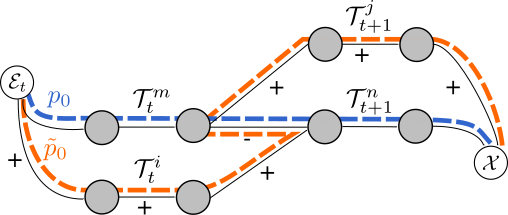
\includegraphics[width=0.49\textwidth]{figa14a}
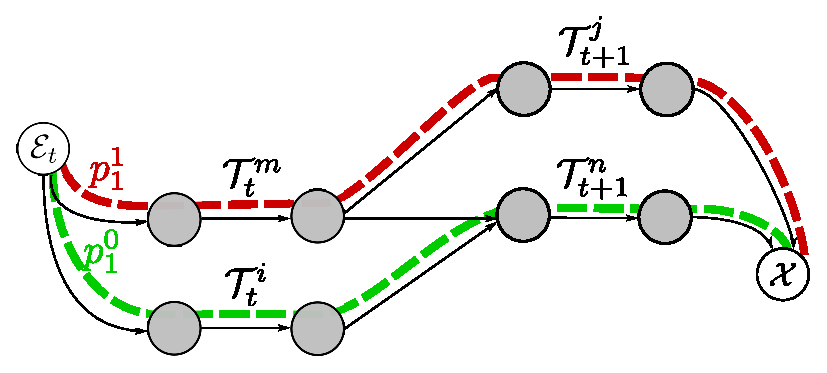
\includegraphics[width=0.49\textwidth]{figa14b}
\caption{Illustration of the interlacing and augmentation procedure for $K$=2. (Left) $p_0$ is the (single) shortest-path of set $P_0$. $\tilde{p}_0$ is the shortest interlacing path obtained after inverting the direction and algebraic sign of edge costs of $P_0$. Positive and negative labels are assigned to the edges of $P_0$. (Right) The optimal set $P_1=\{ p_1^0,p_1^1 \}$ is obtained by removing the edges with negative labels from $p_0$, and adding positive labels.}\label{fig:augment}
\end{figure}


\begin{algorithm}[t]
\caption{K-shortest paths algorithm.\label{alg:ksp}}
\begin{algorithmic}[1]
\Require{$G$: Directed Acyclic Graph constructed as in Sec.~\ref{sec:solving}}
\Ensure{$P$: Set of K-shortest paths}
\State $p_0 \gets$ \texttt{bellman\_ford\_shortest\_paths}$(G)$
\State $P_0 \gets\{p_0\} $
\For{$l\gets 0$ to $l_{max}$ }
 \If{$l \neq 0$}
   \If{\texttt{cost}$(P_l) \geq$ \texttt{cost}$(P_{l-1})$}
     \Return $P_{l-1}$
 \EndIf
 \EndIf
   \State $G_r \gets$ \texttt{reverse}$(G,P_l)$\Comment{Reverse edges directions and algebraic signs}
   \State $G_r^+ \gets$ \texttt{edge\_costs\_transform}$(G_r)$\Comment{As in Eq.~\eqref{eq:cost_transform}}
   \State $\tilde{p}_l \gets$ \texttt{dijkstra\_shortest\_paths}$(G_r^+)$\Comment{Returns interlacing path}
   \State $P_{l+1} \gets$ \texttt{augment}$(P_l, \tilde{p}_l)$\Comment{As on Fig.~\ref{fig:augment}}
\EndFor

\end{algorithmic}
\end{algorithm}
% \end{subappendices}

%%% Local Variables:
%%% mode: latex
%%% TeX-master: "../../main"
%%% End:
